\documentclass[12pt,a4 paper]{article}
\usepackage{ryan}
\usepackage{appendix}
\pgfplotsset{compat=newest}
\renewcommand*{\arraystretch}{1.5}

\begin{document}
\title{\textbf{H2 Chemistry\\ Physical Chemistry}}
\author{Ryan Joo}

\maketitle

\begin{abstract}
This book is written with the intention to provide readers with a brief summary of each topic in the Singapore GCE A-Level Chemistry at the H2 Level. The full syllabus can be found \href{https://www.seab.gov.sg/docs/default-source/national-examinations/syllabus/alevel/2024syllabus/9729_y24_sy.pdf}{here}.
\end{abstract}
\pagebreak

\tableofcontents
\pagebreak

\section{Mole Concept and Stoichiometry}
\subsection{Relative masses}
\begin{defn}{Relative isotopic mass}{}
Mass of one atom of isotope of element relative to $\frac{1}{12}$ of mass of \ce{C-12} atom.
\end{defn}

\begin{defn}{Relative atomic mass $A_r$}{}
Average mass of atoms of element in isotopic mixture relative to $\frac{1}{12}$ of mass of \ce{C-12} atom.
\end{defn}

Given $i$ isotopes, $A_r$ is the weighted average of all isotopes (so it is usually not an integer).
\begin{equation}
A_r = \frac{\sum_i m_i \times \text{Abundance}_i}{\sum_i \text{Abundance}_i}
\end{equation}

\begin{defn}{Relative molecular mass $M_r$}{}
Average mass of one molecule relative to $\frac{1}{12}$ of mass of \ce{C-12} atom.
\end{defn}

$M_r$ is the sum of the $A_r$ of the atoms shown in the molecular formula.
\begin{equation}
M_r = \sum_i (A_r)_i
\end{equation}

\begin{defn}{Relative formula mass $M_r$}{}
Average mass of one formula unit of substance relative to $\frac{1}{12}$ of mass of \ce{C-12} atom.
\end{defn}

\begin{remark}
A formula unit is the smallest collection of atoms from which the formula of an ionic compound can be established. It is equal to the sum of the $A_r$ of the atoms shown in the formula unit.
\end{remark}

\begin{exercise}{}{}
Determine the $A_r$ of chlorine given that there exist two isotopes, \ce{^{35}Cl} and \ce{^{37}Cl}, with percentage isotopic abundance 75\% and 25\%, respectively.
\end{exercise}

\begin{solution}
To calculate $A_r$, we need to consider the relative amount of each isotope. To calculate a weighted average,
\[ A_r\text{ of chlorine} = \frac{75(35)+25(37)}{75+25} = \boxed{35.5} \]
\end{solution}

\subsection{Mole}
\begin{defn}{Mole}{}
One mole contains exactly $6.02 \times 10^{23}$ (or Avogadro constant) elementary entities.
\end{defn}

Avogadro constant $L=6.02 \times 10^{23}\,\unit{mol^{-1}}$ 

\begin{defn}{Molar mass}{}
Mass of one mole of substance.
\end{defn}

\begin{defn}{Avogadro’s Law}{}
Equal volumes of all gases, under same conditions of temperature and pressure, contain same number of molecules/ atoms.
\end{defn}

\begin{defn}{Molar volume}{}
Volume occupied by one mole of gas.
\end{defn}

Molar volume at r.t.p. = $24.0\,\unit{dm^3\,mol^{-1}}$

Molar volume at s.t.p. = $22.7\,\unit{dm^3\,mol^{-1}}$

\begin{defn}{Standard solution}{}
Solution which contains known amount of solute in given volume of solution (i.e. one with a known concentration).
\end{defn}

Dilution:
\begin{equation}
C_0V_0 = C_dV_d
\end{equation}

\subsection{Oxidation number}
Rules to assign oxidation number
\begin{enumerate}
\item ON of element = 0
\item ON of H in compound = +1 (except in metal hydrides)
\item ON of O in compound = -2 (except in peroxides, superoxides)
\item ON of more electronegative atom = -ve
\item ON of less electronegative atom = +ve
\item ON of uncharged compound = sum of individual ON = 0
\end{enumerate}

\subsection{Redox reactions}
To construct a redox equation in acidic medium,
\begin{enumerate}
\item Construct unbalanced oxidation and reduction half-equations
\item Balance all elements except \ce{H} and \ce{O}
\item Balance \ce{O} atoms by adding \ce{H2O}
\item Balance \ce{H} atoms by adding \ce{H+} ions
\item Balance charges by adding electrons
\item Add both half-equations
\end{enumerate}

To construct a redox equation in alkaline medium,
\begin{enumerate}[resume]
\item Neutralise \ce{H+} ions by adding \ce{OH-} ions, combine \ce{H+} and \ce{OH-} to form \ce{H2O}
\end{enumerate}

\subsubsection{Half equations}
\textbf{Manganate(VII)} as oxidising agent
\[ \ce{MnO4^- + 8 H^+ + 5 e^- -> Mn^2+ + 4 H2O} \]
\textbf{Dichromate(VI)} as oxidising agent
\[ \ce{Cr2O7^2- + 14 H^+ + 6 e^- -> 2 Cr^3+ + 7 H2O} \]
\textbf{Thiosulfate} as reducing agent
\[ \ce{I2 + 2 S2O3^2- -> 2 I^- + S4O6^2-} \]

Calculate empirical and molecular formulae

Back-titration

\subsection{Combustion}
Complete combustion of hydrocarbon:
\begin{center}
\ce{C_xH_y + $\brac{x+\dfrac{y}{4}}$ O2(g) -> $x$ CO2(g) + $\dfrac{y}{2}$ H2O(l)}
\end{center}
\pagebreak
\section{Atomic Structure}
\subsection{Subatomic particles}
\begin{table}[H]
\centering
\begin{tabular}{cccc}
\hline\hline
\textbf{particle} & \textbf{charge} & \textbf{mass} & \textbf{angle of deflection} \\
\hline
proton & $+1$ & $1$ & small \\
electron & $-1$ & $\approx 0$ & large \\
neutron & $0$ & $1$ & none \\
\hline\hline
\end{tabular}
\caption{Subatomic particles}
\end{table}

\subsubsection{Behaviour in an electric field/magnetic field}
Deflection of subatomic particles in electric field:
\begin{equation}
\angle \propto \frac{q}{m} \iff \angle = k\frac{q}{m}
\end{equation}
\begin{remark}
Constant of proportionality $k$ remains the same under the same experimental conditions.
\end{remark}
\begin{remark}
Note the sign of charge $q$: electrons and protons are deflected in opposite directions.
\end{remark}

A beam of charged particles passing through an electric field is deflected.
\begin{figure}[H]
    \centering
    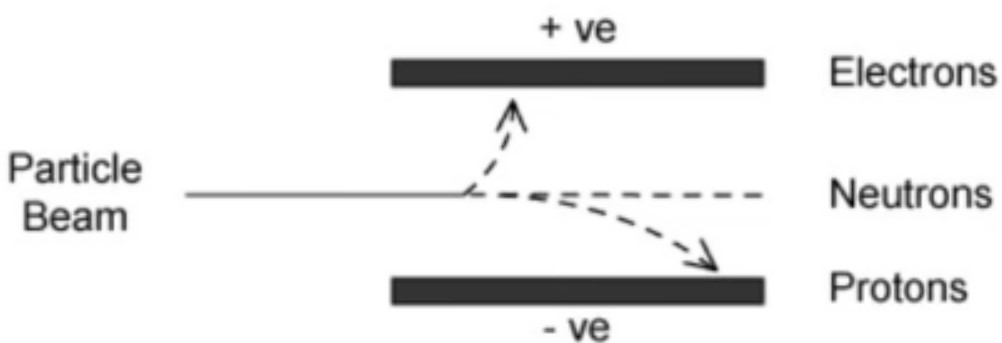
\includegraphics[width=10cm]{images/sub_particle_deflectn.jpg}
    \caption{Deflection of subatomic particles in electric field}
\end{figure}

\subsubsection{Isotopes}

\begin{defn}{Isotope}{}
Atom of same element with same number of protons but different number of neutrons.
\end{defn}

Isotopes have similar chemical properties since they have the same number of protons and hence the same number of electrons. 

However, their physical properties differ since they have different numbers of neutrons and hence different masses.

To distinguish among the isotopes present, a classification system has been devised. In this system, the nuclide of an element is represented as such:
\[ ^A_Z X \]
where $X$ denotes atomic symbol of the element in the periodic table, $Z$ denotes the atomic number/proton number (number of protons in the nucleus), $A$ denotes mass number/nucleon number (number of protons and neutrons in the nucleus).

\subsection{Electronic structure}

\begin{defn}{Orbital}{}
Region in space where there is high probability of finding an electron.
\end{defn}



\subsection{Electronic configuration}
\textbf{Ground state}: electron occupy orbitals of lowest available energy levels

\textbf{Excited state}: electron absorbs energy, promoted to higher energy level. Such atoms are unstable, release energy to return to ground state

Rules of orbital filling
\begin{enumerate}
\item \textbf{Aufbau principle}

Electrons occupy lowest energy orbitals first before higher energy orbitals -- filled in the order of increasing orbital energy.
(4s filled before, removed before 3d)

\item \textbf{Hund's rule}

Electrons added into orbitals singly first with parallel spins before pairing. 
(electrons positioned as far apart as possible to minimise inter-electronic repulsion)

\item \textbf{Pauli exclusion principle}

Each orbital holds max 2 electrons in opposite spins.
\end{enumerate}

Exceptions\footnote{You need to know these!}:
\begin{itemize}
\item \textbf{Chromium}: [Ar]$\unit{3d^5\,4s^1}$ instead of [Ar]$\unit{3d^4\,4s^2}$

to minimise inter-electronic repulsion

\item \textbf{Copper}: [Ar]$\unit{3d^{10}\,4s^1}$ instead of [Ar]$\unit{3d^9\,4s^2}$

fully filled 3d shells are stable due to symmetrical charge distribution
\end{itemize}


\subsection{Atomic trends}
\begin{defn}{First ionisation energy}{}
Energy required to remove 1 mole of electrons from 1 mole of gaseous atoms of the element to form 1 mole of singly charged gaseous cations.
\end{defn}

\begin{defn}{Second ionisation energy}{}
Energy required to remove 1 mole of electrons from 1 mole of singly positively charged gaseous ions to form 1 mole of doubly charged gaseous cations.
\end{defn}

\begin{defn}{Nuclear charge}{}
Electrostatic attraction of protons in nucleus on surrounding electrons.
\end{defn}

\begin{defn}{Shielding effect}{}
Partial decrease in electrostatic attraction of nucleus on valence electrons due to repulsive forces from other electrons.
\end{defn}

\begin{defn}{Effective nuclear charge}{}
Net electrostatic attraction of protons in nucleus on valence electrons.
\end{defn}
\pagebreak
\section{Chemical Bonding}
\subsection{Types of Bonding}
\begin{table}[H]
\centering
\begin{tabular}{p{3cm}p{7cm}p{5cm}}
\hline\hline
\textbf{Type} & \textbf{Description} & \textbf{Factors affecting bond strength} \\
\hline
\vocab{Ionic bond} & Electrostatic forces of attraction b/w oppositely charged ions in giant ionic structure & Lattice energy $\propto \dfrac{q^+ \cdot q^-}{r^++r^-}$ \\
\vocab{Metallic bond} & Electrostatic forces of attraction b/w lattice of cations \& sea of delocalised electrons in giant metallic structure & No. of valence electrons available for delocalisation per atom

Size of metal cation (cationic radius) \\
\vocab{Covalent bond} & Electrostatic forces of attraction b/w positively charged nuclei of two atoms \& shared pair of electrons in simple/giant molecular structure (formed due to orbital overlap) & Bond dissociation energy, affected by:

Bond order (no. of bonds)
Effectiveness of orbital overlap: 
larger orbital is more diffused → orbital overlap less effective → shorter bond length → weaker bond strength
Bond length: sigma bond vs pi bond
Polar VS non-polar bond
 \\
\vocab{Dative bond} & Electrostatic forces of attraction b/w positively charged nuclei of donor and acceptor atom \& shared pair of electrons 
\begin{itemize}
\item \textbf{Donor}: lone pair of electrons available for donation (electron-rich)
\item \textbf{Acceptor}: vacant low-lying orbital to accept electron pair (electron-deficient)
\end{itemize} &  \\
\hline\hline
\end{tabular}
\end{table}

\begin{defn}{Electronegativity}{}
Ability of atom to attract shared pair of electrons towards itself in a covalent bond.
\end{defn}

Intermediate bond types

\subsection{Covalent Bonds}
\subsubsection{Overlap of orbitals}
\subsubsection{Polarity}
• Bond polarities and polarity of molecules
\subsubsection{Octet rule}
\subsubsection{Valence Shell Electron Pair Repulsion (VSEPR) theory}
• Shapes of simple molecules and bond angles

\subsection{Intermolecular Forces}
\begin{defn}{Instantaneous dipole-induced dipole interaction}{}
Electrostatic forces of attraction b/w oppositely charged poles ($\delta+$ and $\delta-$) of temporary dipoles in molecules.
\end{defn}

\begin{defn}{Permanent dipole-permanent dipole interaction}{}
Electrostatic forces of attraction b/w oppositely charged poles ($\delta+$ and $\delta-$) of permanent dipoles in polar molecules
\end{defn}

\begin{defn}{Hydrogen bond}{}
Electrostatic forces of attraction b/w molecules in simple molecular substances involving hydrogen atom from H-F/O/N covalent bond \& lone pair from F/O/N of another molecule
\end{defn}

\subsection{Physical Properties}

\pagebreak


\section{Gaseous State}
\subsection{Gas Laws}
The gas laws are given by
\begin{itemize}
\item \textbf{Boyle's Law}: $p \propto \dfrac{1}{V}$ at constant $T$ and $n$
\item \textbf{Charles' Law}: $V \propto T$ at constant $p$ and $n$
\item \textbf{Gay--Lussac's Law}: $p \propto T$ at constant $V$ and $n$
\item \textbf{Avogadro's Law}: $V \propto n$ at constant $p$ and $n$
\end{itemize}

\begin{remark}
Remember to take note which quantities are \emph{variables} and \emph{constants}!
\end{remark}

\begin{remark}
SI units must be used for calculations: $p$ (in Pa), $T$ (in K), $V$ (in $\unit{m^3}$), $n$ (in mol)

Note that 1 atm = 101325 Pa, 1 bar = $10^5$ Pa, T (K) = T (\degree C) + 273
\end{remark}

\subsubsection{Ideal gas equation}
The \vocab{ideal gas equation} is given by
\begin{equation}\label{eqn:ideal_gas}
pV = nRT
\end{equation}
where molar gas constant $R = 8.31 \unit{J\,K^{-1}\,mol^{-1}}$

From \cref{eqn:ideal_gas} we can derive the expression for \textbf{molar mass} of gas:
\begin{equation}
M_r = \frac{mRT}{pV}
\end{equation}

and also the expression for \textbf{density} of gas:
\begin{equation}
\rho = \frac{pM_r}{RT}
\end{equation}

\subsubsection{Partial pressure}
\begin{defn}{Dalton's Law}{}
In a mixture of inert gases at constant volume and temperature, total pressure of mixture is the sum of partial pressures of constituent gases.
\end{defn}

\begin{equation}
p_\text{gas} = \frac{n_\text{gas}}{n_T}p_T
\end{equation}

\subsection{Kinetic theory of gases}
Basic assumptions:
\begin{enumerate}
\item Small particles of negligible volumes, as compared to container
\item Negligible intermolecular forces of attraction
\item Perfectly elastic collisions between gas particles and walls of container
\end{enumerate}

All gases are non-ideal; they are real gases.
\begin{table}[H]
\centering
\begin{tabular}{p{7.5cm}p{7.5cm}}
\hline\hline
\textbf{Approach ideality} & \textbf{Deviate from ideality} \\
\hline
High temperature: gas particles able to overcome most of the intermolecular forces of attraction & Low temperature: molecules move more slowly, intermolecular forces of attraction become less negligible \\
\hline
Low pressure: volume of gas particles becomes negligible as compared to volume occupied by gas & High pressure: intermolecular distances become less negligible \\
\hline
& Strong intermolecular forces of attraction

Large size of gas molecule \\
\hline\hline
\end{tabular}
\end{table}

\begin{defn}{Compressibility}{}
Ratio of measured molar volume $V_m$ to molar volume of ideal gas $V_m^\circ$ at same temperature and pressure.
\begin{equation}
Z = \frac{V_m}{V_m^\circ} = \frac{pV_m}{RT}
\end{equation}
\end{defn}

\subsubsection{Compressibility against pressure}
[graph]

At low pressure, $Z<1$. Reason: Attractive forces between molecules, molar volume $V_m$ is smaller than that of ideal gas $V_m^\circ$.

At high pressure, $Z>1$. Reason: Repulsive forces between molecules, molar volume $V_m$ is larger than that of ideal gas $V_m^\circ$.

\subsubsection{Compressibility against temperature}
[graph]

Temperature decreases, deviation from ideality increases
Average kinetic energy of gas particles decreases
Gas particles closer together, intermolecular forces of attraction become significant 
$V_m$ smaller than that of ideal gas

\pagebreak


\section{Chemical Energetics}
\subsection{Thermochemistry}
\begin{defn}{Enthalpy change of reaction $\Delta H$}{}
Energy change when molar quantities of reactants as specified by the chemical equation react to form products.
\end{defn}

\begin{defn}{Hess' Law}{}
Enthalpy change accompanying a chemical reaction is the same regardless of the route by which the chemical change occurs, provided the initial and final states are the same.
\end{defn}

\begin{defn}{Standard enthalpy change of reaction $\Delta H\stst$}{}
Energy change when molar quantities of reactants as specified by the chemical equation react to form products at standard conditions.
\end{defn}

\begin{defn}{Standard enthalpy change of formation $\Delta H_f\stst$}{}
Energy change when one mole of the substance is formed from its constituent elements under standard conditions.
\[ \ce{Na (s) + 1/2 Cl2(g) -> NaCl (s)} \]
\end{defn}

\begin{equation}
\Delta H=\sum H_f\text{ (products)}-\sum H_f\text{ (reactants)}
\end{equation}

\begin{defn}{Standard enthalpy change of combustion $\Delta H_c\stst$}{}
Energy evolved when one mole of the substance is completely burnt in oxygen under standard conditions.
\[ \ce{CH4(g) + 2 O2(g) -> CO2(g) + 2 H2O(l)} \]
\end{defn}

\begin{equation}
\Delta H=\sum H_c\text{ (reactants)}-\sum H_c\text{ (products)}
\end{equation}

\begin{defn}{Standard enthalpy change of hydration $\Delta H_{\mathrm{hyd}}\stst$}{}
Energy evolved when one mole of gaseous ions is hydrated under standard conditions
Standard enthalpy change of solution.
\[ \ce{Na^+(g) -> Na^+(aq)} \]
\end{defn}

\begin{equation}
\Delta H_\text{hyd}\stst\propto\frac{q^+}{r^+}
\end{equation}

\begin{defn}{Standard enthalpy change of solution $\Delta H_{\mathrm{soln}}\stst$}{}
Energy change when one mole of substance is completely dissolved in a solvent to form an infinitely dilute solution under standard conditions.
\[ \ce{NaCl (s) -> Na^+(aq) + Cl^-(aq)} \]
\end{defn}

\begin{defn}{Standard enthalpy change of neutralisation $\Delta H_n\stst$}{}
Energy evolved when one mole of water is formed from the neutralisation between acid and base under standard conditions.
\[ \ce{H^+(aq) + OH^-(aq) -> H2O(l)} \]
\end{defn}

\begin{defn}{Standard enthalpy change of atomisation $\Delta H_{\mathrm{atom}}\stst$}{}
Energy absorbed when one mole of gaseous atoms is formed from the element under standard conditions.
\[ \ce{1/2 Cl2(g) -> Cl(g)} \]
\end{defn}

\begin{defn}{Bond dissociation energy}{}
Energy required to break one mole of covalent bond in a specific molecule in the gaseous state to form gaseous atoms.
\end{defn}

\begin{defn}{Bond energy}{}
Average energy absorbed to break one mole of covalent bond in the gaseous state to form gaseous atoms under standard conditions.
\end{defn}

\begin{equation}
\Delta H\stst=\sum\text{BE (bonds broken)}-\sum\text{BE (bonds formed)}
\end{equation}

\begin{equation}
\text{BE (\ce{A2})}=2\Delta H_\text{atom}\stst\text{ (\ce{A2})}
\end{equation}

\begin{defn}{First ionisation energy}{}
Energy absorbed when one mole of gaseous atoms loses one mole of electrons to form one mole of singly charged gaseous cations.
\[ \ce{Na(g) -> Na^+(g) + e^-} \]
\end{defn}

\begin{defn}{Second ionisation energy}{}
Energy absorbed when one mole of singly charged gaseous cations loses one mole of electrons to form one mole of doubly charged gaseous cations.
\[ \ce{Mg^+(g) -> Mg^2+(g) + e^-} \]
\end{defn}

\begin{defn}{First electron affinity}{}
Energy evolved when one mole of gaseous atoms acquires one mole of electrons to form one mole of singly charged gaseous anions.
\[ \ce{Cl(g) + e^- -> Cl^-(g)} \]
\end{defn}

\begin{defn}{Second electron affinity}{}
Energy absorbed when one mole of singly charged gaseous anions acquires one mole of electrons to form one mole of doubly charged gaseous anions.
\[ \ce{S^-(g) + e^- -> S^2-(g)} \]
\end{defn}

\begin{defn}{Lattice energy}{}
Energy evolved when one mole of the solid ionic compound is formed from its constituent gaseous ions under standard conditions.
\[ \ce{Na^+(g) + Cl^-(g) -> NaCl (s)} \]
\end{defn}

\begin{equation}
\text{LE}\propto\frac{q^+\cdot q^-}{r^++r^-}
\end{equation}

\begin{equation}
\Delta H_\text{soln}\stst=\sum\Delta H_\text{hyd}\stst-\text{LE}
\end{equation}

\begin{remark}
Take note of the following when writing equations:
\begin{enumerate}
\item State symbols
\item Stoichiometric coefficients
\item Sign for $\Delta H$
\end{enumerate}
\end{remark}

\begin{ebox}
\textbf{Values}
\begin{itemize}
\item Standard conditions: 298 K, 1 bar 
\item Standard temperature and pressure (s.t.p.): 273 K, 1 atm
\item Room temperature: $20\degree C$
\item Specific heat capacity of water: $4.18 \unit{kJ.kg.{-1}.K^{-1}}$ (or $4.18 \unit{J.g^{-1}.K^{-1}}$)
\end{itemize}
Refer to Data Booklet for bond energies, ionisation energies.
\end{ebox}

\subsubsection{Heat change}
\begin{equation}
Q=mc\Delta T
\end{equation}

\begin{equation}
\Delta H=\pm\frac{Q}{n}
\end{equation}

\subsection{Thermodynamics}
\begin{defn}{Entropy $S$}{}
Degree of disorder or randomness in a system.
\end{defn}

Factors affecting entropy change $\Delta S$:
\begin{itemize}
\item \textbf{Temperature} 

At higher temperature, average kinetic energy of particles increases. More ways to distribute greater amount of energy among particles. Entropy increases.

\item \textbf{Phase}

Particles move about more freely and with greater speeds. More ways to distribute particles and energy. Entropy increases.

\item \textbf{Number of particles}

More particles moving randomly. More ways to distribute particles and energy. Entropy increases.

\item \textbf{Expansion of volume} (gaseous system)

Larger volume. More ways to distribute particles and energy. Entropy increases.

\item \textbf{Mixing of particles}

When gases are mixed, each gas expands to occupy the whole container. More ways to distribute particles and energy in a larger volume. Entropy increases.
\end{itemize}

\subsubsection{Spontaneity}
\textbf{Gibbs free energy change} $\Delta G$ is given by
\begin{equation}
\Delta G = \Delta H - T \Delta S
\end{equation}

\begin{remark}
Note that since the units of $\Delta S$ is usually given in $\unit{J\,mol^{-1}\,K^{-1}}$, so it has to be converted to $\unit{kJ\,mol^{-1}\,K^{-1}}$ for calculations of $\Delta G$.
\end{remark}

Standard Gibbs free energy change, at standard conditions, is given by
\[ \Delta G\stst = \Delta H\stst - T \Delta S \]

The spontaneity of a reaction can be determined from the value of $\Delta G$:
\begin{table}[H]
\centering
\begin{tabular}{|c|c|}
\hline
$\Delta G < 0$ & Reaction is spontaneous \\
\hline
$\Delta G > 0$ & Reaction is non-spontaneous \\
\hline
$\Delta G = 0$ & Reaction is at equilibrium (phase change) \\
\hline
\end{tabular}
\end{table}

To determine the change in spontaneity of reaction with temperature, use the \textbf{signs} of $\Delta H$ and $-T\Delta S$ to determine change in $\Delta G$.\footnote{sketch out graph to visualise better}

\begin{table}[H]
\centering
\begin{tabular}{ccccc}
\hline\hline
$\Delta H$ & $\Delta S$ & $-T\Delta S$ & $\Delta G$ & Spontaneity \\
\hline
$-$ & $+$ & $-$ & always negative & Spontaneous at ALL temperatures \\
$+$ & $-$ & $+$ & always positive & Non-spontaneous at ALL temperatures \\
$+$ & $+$ & $-$ & negative if $|T\Delta S| > |\Delta H|$ & Spontaneous at HIGH temperatures \\
$-$ & $-$ & $+$ & negative if $|\Delta H| > |T\Delta S|$ & Spontaneous at LOW temperatures \\
\hline\hline
\end{tabular}
\end{table}





Limitations in the use of $\Delta G$ to predict spontaneity:
\begin{itemize}
\item Kinetic feasibility

Some reactions are energetically feasible (also known as thermodynamically feasible) since $\Delta G$ is negative, but kinetically not feasible since it occurs very slowly due to high activation energy. Such reactions are spontaneous but very slow.

\item Non-standard conditions

$\Delta G\stst$ can only be used to predict the spontaneity of a reaction under standard conditions. Under non-standard conditions, $\Delta G$ must be calculated.
\end{itemize}

\pagebreak


\section{Chemical Equilibria}
\subsection{Dynamic equilibrium}
\begin{defn}{Dynamic equilibrium}{}
The state of a reversible process at which the rates of forward and backward reactions are equal, but not equal to zero.

No change in concentrations of reactants and products, i.e. $k_f=k_b$.
\end{defn}

\subsection{Equilibrium Law and Equilibrium Constants}

\subsubsection{Equilibrium constants}
For a reaction with equation \ce{aA + bB <=> cC + dD}, the equilibrium constant, in concentrations, is given by
\begin{equation}
K_C = \frac{[C]^c[D]^d}{[A]^a[B]^b}
\end{equation}

In pressures, the equilibrium constant is given by
\begin{equation}
K_p = \frac{{P_C}^c{P_D}^d}{{P_A}^a{P_B}^b}
\end{equation}

\begin{equation}
K_C=\frac{k_f}{k_b}
\end{equation}

Recall that the partial pressure of gas is given by
\begin{equation}
P_A=\frac{n_A}{n_T}P_T
\end{equation}

Degree of dissociation of A
\begin{equation}
\alpha=\frac{n_{A,\text{dissociated}}}{n_{A,\text{initial}}}
\end{equation}

The position of equilibrium is related to $K_C$.
\begin{table}[H]
\centering
\begin{tabular}{|p{2cm}|p{11cm}|}
\hline
$K_C>1$ & More products at equilibrium,

reaction proceeds in forward direction to larger extent,

POE lies to the right. \\
\hline
$K_C<1$ & More reactants at equilibrium,

reaction proceeds in backward direction to larger extent,

POE lies to the left. \\
\hline
\end{tabular}
\end{table}

To do calculations, use the \textbf{ICE table}.
\begin{table}[H]
\centering
\begin{tabular}{|c|c|c|c|c|}
\hline
& A & B & C & D \\
\hline
Initial moles / mol & & & & \\
\hline
Change in moles / mol & & & & \\
\hline
Equilibrium moles / mol & & & & \\
\hline
\end{tabular}
\end{table}

\begin{remark}
Note when to use moles, concentration, or partial pressure; use moles when total pressure is not constant.
\end{remark}

Gibbs free energy change
\begin{table}[H]
\centering
\begin{tabular}{|p{2cm}|p{11cm}|}
\hline
$\Delta G<0$ & Forward is spontaneous

$K > 1$, POE lies to right \\
\hline
$\Delta G=0$ & Equilibrium

$K = 1$ \\
\hline
$\Delta G>0$ & Backward is spontaneous

$K < 1$, POE lies to left \\
\hline
\end{tabular}
\end{table}

\subsection{Le Chatelier's Principle}

\begin{defn}{Le Chatelier’s Principle}{}
If a system at dynamic equilibrium is subjected to a change which disturbs the equilibrium, the system responds in such a way so as to counteract the effect of the change to re-establish equilibrium.
\end{defn}

Change in concentration
Change in pressure
Change in temperature
Addition of catalyst

\subsection{Haber Process}
\[ \ce{N2(g) + 3 H2(g) <=> 2 NH3(g)} \]

\begin{table}[H]
\centering
\begin{tabular}{p{7.5cm}p{7.5cm}}
\hline\hline
\textbf{Temperature} & \textbf{Pressure} \\
\hline
Expectation: reaction is favoured by low temperature & Expectation: reaction is favoured by high pressure \\
\hline
Reality: High temperature used for higher rate of reaction, economical production & Reality: Low pressure used, as high cost of maintaining equipment for high pressure \\
\hline\hline
\end{tabular}
\end{table}
\pagebreak


\section{Chemistry of Aqueous Solutions}
\subsection{Theories of Acids and Bases}
\begin{table}[H]
\centering
\begin{tabular}{p{2cm}p{6.5cm}p{6.5cm}}
\hline\hline
Theory & \textbf{Acid} & \textbf{Base} \\
\hline
\vocab{Arrhenius} & hydrogen-containing substance, ionises and releases \ce{H+} ions in aq solution & hydroxide-containing substance, ionises and releases \ce{OH-} ions in aq solution \\
\vocab{Br{\o}nsted--Lowry} & proton donor & proton acceptor \\
\vocab{Lewis} & electron pair acceptor (electrophile) & electron pair donor (nucleophile) \\
\hline\hline
\end{tabular}
\end{table}

\begin{remark}
Let $A$ denote the set of Arrhenius acids and bases, $B$ denote the set of Br{\o}nsted--Lowry acids and bases, $L$ denote the set of Lewis acids and bases. Then
\[ A \subset B \subset L. \]
\end{remark}

\subsubsection{Conjugate acid-base pair}
\vocab{Conjugate acid-base pair}: a pair of compounds or ions which \emph{differ by one proton}
\begin{itemize}
\item When acid \ce{HA} donates proton to base, conjugate base \ce{A-} is formed.
\[ \ce{HA <=> A- + H+} \]
\item When base \ce{B} receives proton from acid, conjugate acid \ce{BH+} is formed.
\[ \ce{B + H+ <=> BH+} \]
\end{itemize}
Conjugate acid-base pairs: \ce{HA} and \ce{A-}, \ce{B} and \ce{BH+}

\subsubsection{Lewis acids}
Types of species which can act as Lewis acids
\begin{itemize}
\item Electron-deficient molecules

Less than an octet of electrons around one atom. Dative bond formed in adduct\footnote{compound that contains a dative bond between the Lewis acid and the Lewis base}.

\item Molecules with central atom that can expand octet

Low-lying vacant orbitals to accept lone pairs of electrons.

\item Molecules with multiple bonds that has atom with partial positive charge

Lewis base donates lone pair of electrons to form bond with central atom, one pair of electrons displaced from multiple bond to become lone pair on terminal atom.

\item Metal cations

Accept lone pair of electrons via dative bond to form complex ions.
\end{itemize}
\pagebreak

\subsection{Acid--Base Equilibria}
\subsubsection{Strength of acids and bases}
\vocab{Strength} is a measure of extent of dissociation to give ions in solution. (independent of concentration)

\begin{table}[H]
\centering
\begin{tabular}{p{4cm}p{5.5cm}p{5.5cm}}
\hline\hline
 & \vocab{Strong} & \vocab{Weak} \\
\hline
Definition & Complete dissociation in aq solution & Partial dissociation in aq solution \\
Extent of dissociation & $100\%$ & $<<100\%$ \\
Arrow & \ce{->} & \ce{<=>} \\
Equilibrium constant & -- & $K_a$, $K_b$ \\
\hline\hline
\end{tabular}
\end{table}

\subsubsection{Acid and base dissociation constants}
\vocab{Power of hydrogen}:
\begin{equation}
pH = -\lg [\ce{H+}]
\end{equation}

\vocab{Power of hydroxide}:
\begin{equation}
pOH = -\lg [\ce{OH-}]
\end{equation}

\vocab{Acid dissociation constant}: measure of strength of \emph{weak} acid\footnote{equilibrium constant}
\begin{equation}
K_a = \frac{[\ce{H+}][\ce{A-}]}{[\ce{HA}]}
\end{equation}

\begin{equation}
pK_a = -\lg K_a
\end{equation}

\vocab{Base dissociation constant}: measure of strength of \emph{weak} base
\begin{equation}
K_b = \frac{[\ce{BH+}][\ce{OH-}]}{[\ce{B}]}
\end{equation}

\begin{equation}
pK_b = -\lg K_b
\end{equation}

Acidic, basic \& neutral solutions
\begin{table}[H]
\centering
\begin{tabular}{cc}
\hline\hline
Solution & Meaning \\
\hline
\textbf{acidic} & $[\ce{H+}]>[\ce{OH-}]$ \\
\textbf{basic} & $[\ce{H+}]<[\ce{OH-}]$ \\
\textbf{neutral} & $[\ce{H+}]=[\ce{OH-}]$ \\
\hline\hline
\end{tabular}
\end{table}

\subsubsection{Ionic product of water}
Self-ionisation of water can be simplified to \ce{H2O(l) <=> H+(aq) + OH-(aq)}.

\vocab{Ionic product of water}:
\begin{equation}
K_w = [\ce{H+}][\ce{OH-}] = 1.0\times10^{-14}\,\unit{mol^2\,dm^{-6}} \text{ at 298 K}
\end{equation}

By manipulation we have
\begin{equation}
pH + pOH = pK_w = 14 \text{ at 298 K}
\end{equation}

The following relationship holds for a conjugate acid-base pair:
\begin{equation}
K_w = K_a K_b
\end{equation}

This suggests a reciprocal strength relationship: the stronger the acid, the weaker its conjugate base (and vice versa).

\subsubsection{Salt solutions}
Salts undergo hydration to form solutions. Then cations / anions undergo hydrolysis to form acidic / alkaline solutions.

\begin{table}[H]
\centering
\begin{tabular}{p{7.5cm}p{7.5cm}}
\hline\hline
\vocab{Acidic salt solution} & \vocab{Alkaline salt solution} \\
\hline
cation: conjugate acid of WB hydrolyses partially in water to give \ce{H3O+} & anion: conjugate base of WA hydrolyses partially in water to give \ce{OH-} \\
\ce{BH+(aq) + H2O(l) <=> B(aq) + H3O+(aq)} & \ce{A-(aq) + H2O(l) <=> HA(aq) + OH-(aq)} \\
\hline\hline
\end{tabular}
\end{table}

\subsubsection{Buffer solutions}
\begin{defn}{Buffer solution}{}
A solution capable of maintaining a fairly constant pH (by resisting pH change) when small amounts of acid or base are added to it.
\end{defn}

\begin{table}[H]
\centering
\begin{tabular}{p{7.5cm}p{7.5cm}}
\hline\hline
\vocab{Acidic buffer solution} & \vocab{Basic buffer solution} \\
\hline
weak acid + salt of conjugate base (\ce{HA} and \ce{A-}) & weak base + salt of conjugate acid (\ce{B} and \ce{BH+}) \\
\hline
On addition of acid:

\ce{A-(aq) + H+(aq) -> HA(aq)} 
& On addition of acid:

\ce{B(aq) + H+(aq) -> BH+(aq)} \\
On addition of base: 

\ce{HA(aq) + OH-(aq) -> A-(aq) + H2O(l)}
& On addition of base:

\ce{BH+(aq) + OH-(aq) -> B(aq) + H2O(l)} \\
\hline
Large reservoir of \ce{HA} and \ce{A-} present is able to cope with small amount of \ce{H+} and \ce{OH-} added. & Large reservoir of \ce{B} and \ce{BH+} present is able to cope with small amount of \ce{H+} and \ce{OH-} added. \\
\hline\hline
\end{tabular}
\end{table}

Buffer solutions are used in systems where pH must not deviate widely. \ce{H2CO3} / \ce{HCO3-} buffer pair is used to control pH of blood:
\[ \ce{H2CO3(aq) <=> H+(aq) + HCO3-(aq)} \]
\begin{itemize}
\item On addition of acid: \ce{HCO3-(aq) + H+(aq) -> H2CO3(aq)}
\item On addition of base: \ce{H2CO3(aq) + OH-(aq) -> HCO3-(aq) + H2O(l)}
\end{itemize}
\pagebreak

\subsubsection{Titration}
Titrate titrant against analyte / Analyte titrated against titrant

\vocab{Equivalence point}: stoichiometric amounts of acid \& base react together

\vocab{End-point}: when indicator first changes colour permanently

Choice of pH indicator is considered appropriate if its pH transition range lies within range of rapid pH change over equivalence point.

pH graph sketching
\begin{enumerate}
\item initial, equivalence, final pH
\item initial, equivalence, final volume
\item buffer region
\end{enumerate}

Types of titration
\begin{itemize}
\item strong acid--strong base

\item strong acid--weak base

\item weak acid--strong base

\item weak acid--weak base
\end{itemize}

(d) describe the changes in pH during acid-base titrations and explain these changes in terms of the strengths of the acids and bases
(e) explain the choice of suitable indicators for acid-base titrations, given appropriate data

\subsubsection{Calculations}
\begin{itemize}
\item \textbf{Water}
\[ \ce{H2O(l) <=> H+(aq) + OH-(aq)} \]
In pure water, $[\ce{H+}]=[\ce{OH-}]$

$K_w=[\ce{H+}][\ce{OH-}]=10^{-14}\,\unit{mol^2\,dm^{-6}}$

$[\ce{H+}]=[\ce{OH-}]=10^{-7}\,\unit{mol\,dm^{-3}}$

\item \textbf{Strong acid}
\[ \ce{H_nA(aq) -> nH+(aq) + A-(aq)} \]
$[\ce{H+}]=n\times[\ce{H_nA}]$

\vspace{5mm}

\textbf{Strong base}
\[ \ce{M(OH)_n(aq) -> M^{n+}(aq) + nOH-(aq)} \]
$[\ce{OH-}]=n\times[\ce{M(OH)_n}]$

\item \textbf{Weak acid} (monobasic)
\[ \ce{HA(aq) <=> A-(aq) + H+(aq)} \]
Since \ce{HA} is weak acid with small $K_a$, assume extent of dissociation of \ce{HA} is negligible, so $[\ce{H+}]$ is so small such that $[\ce{HA}]\approx[\ce{HA}]_\text{initial}$.

$\displaystyle K_a=\frac{[\ce{H+}][\ce{A-}]}{[\ce{HA}]}=\frac{[\ce{H+}]^2}{[\ce{HA}]}\approx\frac{[\ce{H+}]^2}{[\ce{HA}]_\text{initial}}$

\[ \boxed{[\ce{H+}]=\sqrt{K_a\times[\ce{HA}]_\text{initial}}} \]
from which we can calculate $pH$.

\begin{remark}
This formula CANNOT be used to calculate $K_a$ or $[\ce{HA}]_\text{initial}$! Instead use ICE table.
\end{remark}

\vspace{5mm}

\textbf{Weak base} (monoacidic)
\[ \ce{B(aq) + H2O(l) <=> BH+(aq) + OH-(aq)} \]
Since \ce{B} is weak base with small $K_b$, assume extent of dissociation of \ce{B} is negligible, so $[\ce{OH-}]$ is so small such that $[\ce{B}]=[\ce{B}]_\text{initial}$.

$\displaystyle K_b=\frac{[\ce{BH+}][\ce{OH-}]}{[\ce{B}]}=\frac{[\ce{OH-}]^2}{[\ce{B}]}\approx\frac{[\ce{OH-}]^2}{[\ce{B}]_\text{initial}}$
\[ \boxed{[\ce{OH-}]=\sqrt{K_b\times[\ce{B}]_\text{initial}}} \]
from which we can calculate $pOH$ and then $pH$.

\begin{remark}
This formula CANNOT be used to calculate $K_b$ or $[\ce{B}]_\text{initial}$! Instead use ICE table.
\end{remark}

\item \textbf{Acidic salt solution}
\[ \ce{BH+X-(aq) -> BH+(aq) + X-(aq)} \]
\[ \ce{BH+(aq) + H2O(l) <=> B(aq) + H3O+(aq)} \]

\[ \boxed{[\ce{H+}]=\sqrt{K_a\times[\ce{HA}]_\text{initial}}} \]

\vspace{5mm}

\textbf{Alkaline salt solution}
\[ \ce{M+A-(aq) -> M+(aq) + A-(aq)} \]
\[ \ce{A-(aq) + H2O(l) <=> HA(aq) + OH-(aq)} \]

\[ \boxed{[\ce{OH-}]=\sqrt{K_b\times[\ce{B}]_\text{initial}}} \]

\begin{remark}
When solutions are mixed, remember to calculate the new concentrations.
\end{remark}

\item \textbf{Acidic buffer solution}
\[ \boxed{pH = pK_a + \lg\frac{[\ce{A-}]}{[\ce{HA}]}} \]
Maximum buffer capacity: $[\ce{HA}]=[\ce{A-}] \implies pH=pK_a$

\vspace{5mm}

\textbf{Basic buffer solution}
\[ \boxed{pOH = pK_b + \lg\frac{[\ce{BH+}]}{[\ce{B}]}} \]
Maximum buffer capacity: $[\ce{B}]=[\ce{BH+}] \implies pOH=pK_b$

\end{itemize}

Taking -log on both sides gives us
\begin{equation}
pK_a + pK_b = pK_w
\end{equation}
At 298 K, $pK_a+pK_b=14$.

(c) calculate [H+(aq)] and pH values for strong acids, weak monobasic (monoprotic) acids, strong bases, and weak monoacidic bases [Calculations involving weak acids/bases will not require solving of quadratic equations]


\pagebreak

\subsection{Solubility Equilibria}
\begin{defn}{Solubility}{}
\emph{Maximum} mass / amount of solute that can be dissolved per $\unit{dm^3}$ of solvent to produce a \emph{saturated solution} at a given temperature.
\end{defn}

\begin{defn}{Solubility product $K_{sp}$}{}
\emph{Equilibrium constant} which is the product of molar concentrations of dissolved / dissociated ions (each raised to its appropriate power) in a \emph{saturated solution} of salt at a given temperature.
\end{defn}

For a sparingly soluble salt \ce{MX}, \ce{MX (s) <=> M+(aq) + X-(aq)}.
\begin{equation}
K_{sp} = [\ce{M+}]_\text{satn}[\ce{X-}]_\text{satn}
\end{equation}

Factors affecting solubility of salt
\begin{itemize}
\item \textbf{Common ion effect} (addition of cation/anion) 

Reduced solubility of a solute in a solution that already contains the same ion.

Saturated sparingly soluble salt solution \ce{MX} added to soluble salt solution \ce{NaX(aq)} (containing common ion \ce{X-}). $[\ce{X-}]$ increases. By Le Chatelier's Principle, position of equilibrium shifts left to decrease $[\ce{X-}]$, so dissociation of \ce{MX} supressed, \ce{MX} precipitated. Hence solubility decreases in \ce{NaX(aq)} compared to that in water.

\item \textbf{Formation of complex ions} (removal of cation)

Suitable base added to saturated sparingly soluble salt solution \ce{MX}. Formation of complex ions remove cations \ce{M+}, $[\ce{M+}]$ decreases. By Le Chatelier's Principle, position of equilibrium shifts right to increase $[\ce{M+}]$, so dissociation of \ce{MX} favoured. Hence solubility increases.

$[\ce{M+}]$ decreases, ionic product decreases to below $K_{sp}$, so \ce{MX} dissolves.

\item \textbf{pH of solution} (removal of anion)

\ce{H+} added to saturated sparingly soluble salt solution \ce{MOH}. $[\ce{OH-}]$ decreases. By Le Chatelier's Principle, position of equilibrium shifts right to increase $[\ce{OH-}]$. Hence solubility increases.
\end{itemize}

\begin{defn}{Ionic product $\text{IP}$}{}
Product of molar concentrations of constituent ions in solution \emph{at that instant} (each raised to its appropriate power) at a given temperature.
\end{defn}
\begin{equation}
\text{IP} = [\ce{M+}][\ce{X-}]
\end{equation}

Precipitation occurs when $\text{IP}>K_{sp}$.
\begin{table}[H]
\centering
\begin{tabular}{ccc}
\hline\hline
\textbf{Condition} & \textbf{Saturation} & \textbf{Precipitation} \\
\hline
$\text{IP}<K_{sp}$ & Below saturation point (unsaturated) & No \\
$\text{IP}=K_{sp}$ & At saturation point (saturated) & No \\
$\text{IP}>K_{sp}$ & Beyond saturation point (beyond saturation) & Yes \\
\hline\hline
\end{tabular}
\end{table}


Candidates should be able to:
(b) calculate Ksp from concentrations and vice versa
(c) discuss the effects on the solubility of ionic salts by the following:
(i) common ion effect
(ii) formation of complex ion, as exemplified by the reactions of halide ions with aqueous silver ions followed by aqueous ammonia (see also Section 13)

\pagebreak
\section{Electrochemistry}
\subsection{Redox processes}
Oxidation: loss of electrons / increase in oxidation state

Reduction: gain of electrons / decrease in oxidation state

\subsection{Electrode potentials}
\begin{defn}{Standard electrode (redox) potential $E\stst$}{}
Potential 
\end{defn}
(i) standard electrode (redox) potentials, $E\stst$; the redox series
(ii) standard cell potentials, $E_\text{cell}\stst$, and their uses
(iii) batteries and fuel cells

\subsection{Electrolysis}
(i) factors affecting the amount of substance liberated during electrolysis
(ii) the Faraday constant; the Avogadro constant; their relationship
(iii) industrial uses of electrolysis

Learning Outcomes
Candidates should be able to:
(a) describe and explain redox processes in terms of electron transfer and/or of changes in oxidation number
(oxidation state)
(b) define the terms:
(i) standard electrode (redox) potential
(ii) standard cell potential
(c) describe the standard hydrogen electrode
(d) describe methods used to measure the standard electrode potentials of:
(i) metals or non-metals in contact with their ions in aqueous solution
(ii) ions of the same element in different oxidation states
(e) calculate a standard cell potential by combining two standard electrode potential
(f) use standard cell potentials to:
(i) explain/deduce the direction of electron flow from a simple cell
(ii) predict the spontaneity of a reaction
(g) understand the limitations in the use of standard cell potentials to predict the spontaneity of a reaction
(h) construct redox equations using the relevant half-equations (see also Section 13)
(i) state and apply the relationship $\Delta G\stst=-nFE\stst$ to electrochemical cells, including the calculation of $E\stst$

for combined half reactions
(j) predict qualitatively how the value of an electrode potential varies with the concentration of the aqueous ion
(k) state the possible advantages of developing other types of cell, e.g. the H2/O2 fuel cell and improved
batteries (as in electric vehicles) in terms of smaller size, lower mass and higher voltage
(l) state the relationship, F = Le, between the Faraday constant, the Avogadro constant and the charge on the
electron
(m) predict the identity of the substance liberated during electrolysis from the state of electrolyte (molten or
aqueous), position in the redox series (electrode potential) and concentration
(n) calculate:
(i) the quantity of charge passed during electrolysis
(ii) the mass and/or volume of substance liberated during electrolysis
(o) explain, in terms of the electrode reactions, the industrial processes of:
(i) the anodising of aluminium
(ii) the electrolytic purification of copper
\pagebreak

\end{document}
